\documentclass[14pt]{matmex-diploma-custom}
\usepackage{amsthm}
\usepackage{mathtools}
\usepackage{amssymb}
\usepackage{graphicx}
\usepackage{wrapfig}
\usepackage{float}
\usepackage[caption=false]{subfig}
\usepackage{tikz}
\usepackage{pgfplots}
\pgfplotsset{compat=1.9}
\usepackage{multirow}
\usepackage{listings}
\usepackage{url}
\usepackage{algpseudocode}
\usepackage{algorithm}
\usepackage{algorithmicx}
%\documentclass[14pt]{matmex-diploma-custom}
%\hyphenation{Ge-ne-ra-lised}
\newtheorem{mydef}{Определение}
%\tolerance=1
\emergencystretch=\maxdimen
%\hyphenpenalty=10000
%\hbadness=10000
\usetikzlibrary{graphs, graphs.standard, quotes}
\usetikzlibrary{arrows}
\begin{document}
	\renewcommand{\lstlistingname}{Листинг}

	
	% Год, город, название университета и факультета предопределены,
	% но можно и поменять.
	% Если англоязычная титульная страница не нужна, то ее можно просто удалить.
	\filltitle{ru}{
		chair              = {Математическое обеспечение и администрирование\\ информационных систем\\
			\vskip 1em
			Системное программирование},
		title              = {Применение синтаксического анализа в распознавании планов},
		% Здесь указывается тип работы. Возможные значения:
		%   coursework - Курсовая работа
		%   diploma - Диплом специалиста
		%   master - Диплом магистра
		%   bachelor - Диплом бакалавра
		type               = {coursework},
		position           = {студента},
		group              = 546,
		author             = {Горохов Артем Владимирович},
		supervisorPosition = {к.\,ф.-м.\,н., доцент},
		supervisor         = {Григорьев С.\,В.},
		reviewerPosition   = {к},
		reviewer           = {к},
		chairHeadPosition  = {д.\,ф.-м.\,н., профессор},
		chairHead          = {Терехов А.\,Н.}
		%   university         = {Санкт-Петербургский Государственный Университет},
		%   faculty            = {Математико-механический факультет},
		%   city               = {Санкт-Петербург},
		%   year               = {2013}
	}
	\maketitle
	%\setcounter{tocdepth}{1}
	\tableofcontents
	% У введения нет номера главы
	\section*{Введение}
	Интеллектуальные системы получили широкое распространение в современности,
	при этом одним из их важных аспектов является возможность распознавания различных действий людей и других систем.
    Рассмотрим задачу определения цели или планов агента (общеиспользуемый термин), по его действиям. Область науки изучающую 
    этот вопрос называют распознаванием деятельности (Activity recognition). В этой области выделяют различные направления, среди которых
    \textit{распознавание цели~(goal recognition)} и \textit{распознавание планов~(plan recognition)}~\cite{mirsky2017slim},
	основанные на использовании так называемых \textit{библиотек планов} --- наборов схем действий, которым может следовать агент.
    
    \textit{Распознавание цели} --- это задача классификации, цель которой состоит в определении общей цели по выполняемым действиям на основании библиотеки планов.
	Для примера может быть рассмотрен случай наблюдения за действиями человека на кухне. Последовательность действий, начинающаяся
	с ``взбить яйца'', ``смешать с мукой'' может быть распознана как ``выпечка'', ``выпечка торта'', ``выпечка шоколадного торта'' и т. д.
	
	Задача \textit{распознавания планов} включает в себя установление цели, но так же предполагает построение структуры действий согласно
    структуре библиотеки планов. Такой подход предлагает больше данных для последующего анализа.
    В рассмотренном выше примере система, выполняющая распознавание планов, способна в реальном времени выдать
    гипотезу о том, что человек собирается приготовить шоколадный торт. Кроме того, эта же система способна помочь 
    повару предотвратить ошибки, в то время как система, решающая задачу распознавания цели, сможет только переклассифицировать действия с
    ``выпечка шоколадного торта'' на ``неудачная попытка выпечки шоколадного торта''.
    В данной работе будет рассмотрена задача распознавания планов.    
    
    Алгоритмы распознавания планов могут применяться в различных областях: поддержка экипажей по время чрезвычайных ситуаций с помощью распознавания 
    используемого протокола действий~\cite{BlaylockandAllen2006}, уведомление о пропущенных шагах в медицинском руководстве используемым
    врачом~\cite{CharniakandGoldman,NgandMooney1992}, помощь в использовании программного обеспечения в обучении~\cite{AmirandGal2013,Uzan2015}
    и обеспечение реакции в режиме реального времени на кибератаку~\cite{Bisson2011,QinandLee2004}.
	
    Задача распознавания планов связана с синтаксическим анализом: библиотека планов может быть представлена в виде контекстно-свободных грамматик,
    а процесс построения структуры действий --- как построение дерева разбора для грамматики~\cite{maraist2016}. С другой стороны, существуют обстоятельства,
    не позволяющие адаптировать существующие алгоритмы синтаксического анализа для этой области: в распознавании
    планов рассматривают одновременно несколько возможных планов, а так же их чередование (interleaving) в последовательности рассматриваемых действий.
    Таким образом, в большинстве алгоритмов распознавания планов используются идеи синтаксического анализа, но не используются новейшие 
    алгоритмы анализа. Одним из таких алгоритмов является Generalised LL~\cite{scott2010gll}. Данный алгоритм позволяет осуществлять анализ строк
    для произвольных контекстно-свободных грамматик. Кроме того, в лаборатории языковых инструментов Jetbrains, СПбГУ,
    на базе инструмента для создания и изучения синтаксических анализаторов YaccConstructor~\cite{YCUrl}, разработано расширение Generalised LL-алгоритма, позволяющее проводить анализ конечных автоматов, возможночть использования которого представляет интерес.
    %Стоит отметить работу~\cite{maraist2016}, в которой используется алгоритм Generalised LR, но решается задача распознавания цели --- иерархия действий не строится.
	\section{Постановка задачи}
	
	Целью данной работы является создание алгоритма распознавания планов, использующего известные высокопроизводительные алгоритмы синтаксического анализа.
    Для её достижения были поставлены следующие задачи.
	
	\begin{itemize}
		\item Изучить возможность использования алгоритма Generalised LL в решении задачи распознавания планов для получения высокопроизводительного решения.
		\item Разработать новый алгоритм распознавания планов на основе проведённых исследований.
		\item Выполнить реализацию разработанного алгоритма на базе инструмента YaccConstructor.
		\item Провести экспериментальное сравнение реализованного алгоритма с существующими.
	\end{itemize}
		

    
    \section{Обзор}
    \subsection{Распознавание планов}
    Формулировка задачи распознавания планов оперирует понятием библиотеки планов.
    
    \begin{mydef}
    	Библиотека планов --- это кортеж $(\Sigma, NT, R, P)$, состоящий из следующих элементов:
    	\begin{itemize}
    		\item $\Sigma$ и NT --- непересекающиеся конечные алфавиты терминальных действий и нетерминальных целей;
    		\item $R \subseteq NT $ --- множество корневых целей;
    		\item $P$ --- множество продукций вида $(n, \beta, \sqsubset) $, где
    		\begin{itemize}
    			\item $n \in NT$;
    			\item $\beta$ --- строка символов из $ \Sigma \bigcup NT $, для которой $(|\beta| = 1)\&(\beta \subseteq \Sigma)$
    	или $(|\beta| > 1)\&(\beta \subseteq NT)$;
    			\item $ \sqsubset$ --- асимметричное отношение над индексами $[1, |\beta|]$, описывающее допустимый порядок целей.
    		\end{itemize}
    	\end{itemize}
    \end{mydef}
    
    Библиотека планов описывает иерархии которые можно построить из различных действий.
    Задача распознавания планов состоит в построении всех возможных иерархий для наблюдаемых действий, исходддя из информации в библиотека планов.
    При этом на задачу могут накладываться различные ограничения:
    \textit{множества действий в иерархиях не должны пересекаться}; \textit{иерархии должны содержать все наблюдаемые действия} и другие.
     
    
    Во многих задачах необходима работа в реальном времени --- алгоритм строит неполные иерархии действий,
    а с поступлением новых достраивает или отвергает уже построенные. Существующие алгоритмы распознавания планов
    для работы в реальном времени способны обрабатывать только небольшие последовательности действий,
    работать на ограниченных доменах или ограничивать полноту выведенных гипотез~\cite{Kabanza2013,WisemanandShieber2014}.
    Это связано с тем, что
    число гипотез может расти быстро даже для небольшого числа действий~\cite{Mirsky2016}. Как пример этого 
    может быть рассмотрен сценарий выпечки, в котором повар начинает с муки и сахара --- многие рецепты 
    начинаются с этих ингредиентов, поэтому объяснение действий повара потребует генерации большого количества гипотез-иерархий.
    
    \subsection{Контекстно-свободные грамматики с шаффлом}
	Задачу распознавания планов можно рассматривать с точки зрения синтаксического анализа:
	библиотека планов представима набором контекстно-свободных грамматик со стартовыми нетерминалами $R_i$ для каждой корневой
	цели из $R$, 
	а продукции $(n, \beta, \sqsubset) $ --- как продукции грамматики $n \rightarrow \beta'_1 | ... | \beta'_v $,
	где $\beta'_1 ... \beta'_v \in \beta'$ --- 
	все перестановки $\beta$, в которых сохраняется отношение $\sqsubset$. Тогда иерархии --- это деревья разбора последовательностей терминалов (наблюдаемых действий).
	
	В данной работе будет рассмотрена задача распознавания планов с условием, что
	каждое действие принадлежит иерархиям с единой корневой целью. Такая формулировка позволяет строить
	множества непересекающихся иерархий, и рассматривается в последних работах исследующих задачу распознавания планов~\cite{maraist2016,Mirsky2016,mirsky2017slim}.
	Такая постановка задачи также использовалась в работе~\cite{maraist2016}, в которой описывается связь задачи распознавания планов
	с синтаксическим анализом контекстно-свободных грамматик с \textit{шаффлом} (Context-Free Shuffle Grammars, CFSG).
	Для определения CFSG введём понятие \textit{шаффла}.
    
    Операция \textit{шаффла} ($\odot$) строк определяется индуктивно:
    \begin{itemize}
        \item $\epsilon \odot u = u \odot \epsilon = {u}, \forall u \in \Sigma^*$ ($\Sigma$ --- алфавит);
        \item $\alpha_1 u_1 \odot \alpha_2 u_2 = \{\alpha_1 w | w \in (u_1 \odot \alpha_2 u_2) \} \cup
               \{\alpha_2 w | w \in (\alpha_1 u1 \odot u_2 ) \}, \newline \forall \alpha_1, \alpha_2 \in \Sigma$ и $u_1, u_2 \in \Sigma^*$.
    \end{itemize}
    
    Эта операция расширяется на языки следующим образом: \newline $L_1 \odot L_2 = \bigcup\limits_{u_1\in L_1, u_2\in L_2} u_1 \odot u_2$.
    % Для примера рассмотрим следующую грамматику: (TODO)
    
    Единственное структурное отличие контекстно-свободных грамматик с шаффлом (CFSG) от контекстно-свободных грамматик
    --- это структура продукции стартового нетерминала: в CFSG она имеет следующий
    вид: $S = A_1 \odot A_2 \odot ... \odot A_n$
    и задаёт шаффл языков порождаемых нетерминалами $\{A_i | i \in 1..n\}$. %Языки которые CFSG являются контекстно-свободными языками с шаффлом.
    Таким образом, можно осуществить переход от задачи распознавания планов к задаче синтаксического анализа CFSG.%, так так она равнозначна задаче распознавания планов.
    
    \subsection{Построение леса разбора с помощью Generalised LL}
    Одним из наиболее производительных алгоритмов синтаксического анализа контекстно-свободных грамматик является
    Generalised LL (GLL). Данный алгоритм
    позволяет строить деревья разбора строки для любой контекстно-свободной грамматики. Если грамматика неоднозначна
    (возможно несколько вариантов вывода некоторых строк), алгоритм GLL строит все возможные деревья. Для построения используется структура данных Shared Packed Parse Forest (SPPF)~\cite{GLLSPPF}, позволяющая хранить лес разбора (множество деревьев разбора), переиспользуя построенные
    узлы дерева. SPPF содержит следующие типы узлов ($i$ и $j$ --- это начало и конец выведенной подстроки для данного узла).
    
    \begin{itemize}
    	\item \textit{Упакованный узел} $(M, k)$, где $M$ --- позиция в грамматике, $k$ --- начало выведенной
    	подстроки правого ребёнка --- символьного узла. Левый ребёнок опционален и может быть 
    	представлен символьным или промежуточным узлом.
    	\item \textit{Символьный узел} $(X, i, j)$, где $X$ --- терминал или нетерминал.
    	Терминальные символьные узлы --- листья. 
    	\item \textit{Промежуточный узел} $ (M, i, j) $, где $M$ --- позиция в грамматике.
    \end{itemize}

    Символьные и промежуточные узлы имеют 1 или более детей --- упакованных узлов.
    Различные дети этих узлов --- различные варианты выведенных поддеревьев.
    Если у узла (символьного или промежуточного) или его потомков более одного ребёнка, то для него было построено несколько вариантов 
    разбора строки. Так, деревья, представленные на рис.~\ref{fig:Gtrees}, объединяются в SPPF показанный на рис.~\ref{fig:GSPPF}.
    Промежуточные и упакованные узлы необходимы для обеспечения переиспользования узлов SPPF --- такое представление существенно снижает
    затраты памяти для некоторых грамматик, благодаря этому пространственная сложность алгоритма Generalised LL: $O(N^3)$ --- как и временная.
    
    \begin{figure}
    	\centering
    	$
    	\begin{array}[b]{rl}
    	S ::= S\ S\ | \ c \ \ \ 
    	\end{array}
    	$
    	\caption{Неоднозначная грамматика $G_0$}
    	\label{fig:fig0}
    \end{figure}
    \begin{figure}[ht]
    	\centering
    	\subfloat[Возможные деревья вывода]{
    		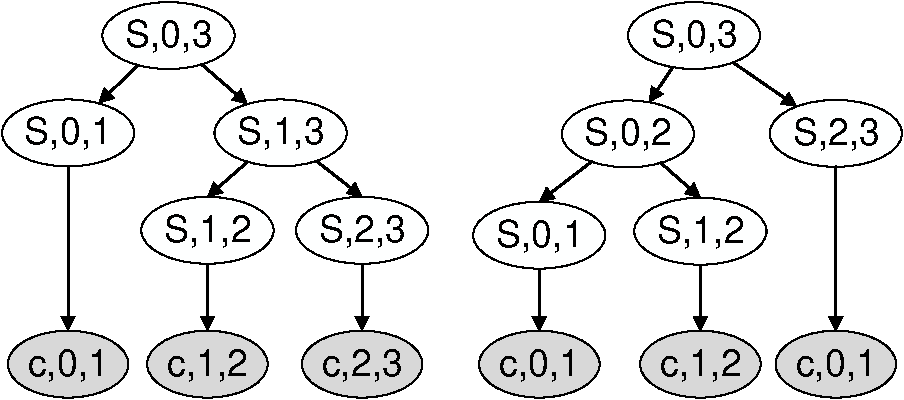
\includegraphics[scale=.6]{pictures/Gtrees.pdf}
    		\label{fig:Gtrees}
    	}
    	~
    	\subfloat[SPPF]{
    		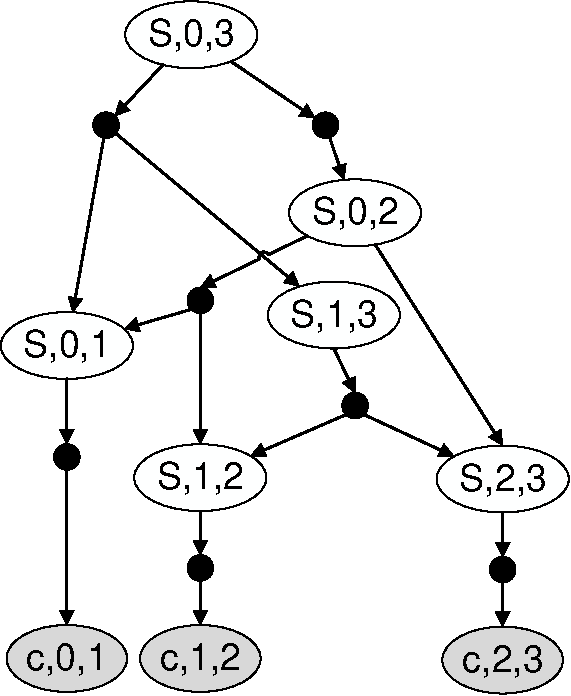
\includegraphics[scale=.6]{pictures/GSPPF.pdf}
    		\label{fig:GSPPF}
    	}
    	\caption{Пример для входа $ ccc $ и грамматики $G_0$}
    	\label{fig:fig01}
    \end{figure}
    
    Кроме того, было предложено расширение алгоритма Generalised LL~\cite{ragozina}, позволяющее для контекстно-свободной
    грамматики производить анализ регулярного множества, представленного в виде конечного автомата. Так, для грамматики
    $S \rightarrow a(b|d)^*cd$ 
    и конечного автомата $M_2$~(рис.~\ref{fig:M2Aut}) алгоритм построит лес разбора, содержащий все строки вида $a b^* cd$.
    Далее будет описано применение этого расширения алгоритма Generalised LL для анализа контекстно-свободных грамматик с шаффлом.
    \begin{figure}[ht]
    	\centering
    	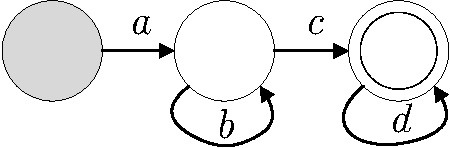
\includegraphics[scale=.6]{pictures/M2Automaton.pdf}
    	\caption{Конечный автомат $M_2$}
    	\label{fig:M2Aut}
    \end{figure}

    \subsection{NP-полнота задачи}
    
    Известно, что задача синтаксического анализа CFSG является NP-сложной~\cite{BERGLUND20131}.
    Одним из известных подходов к решению NP-сложных задач является сведение к задаче выполнимости булевых формул
    (Boolean satisfiability problem, SAT)~\cite{satSolvers}. Задача SAT заключается в определении 
    возможности задания всем переменным, встречающимся в булевой формуле, значения ложь и истина так,
    чтобы формула стала истинной. Для решения
    задачи SAT существует множество так называемых SAT-решателей, и c каждым годом появляются новые работы по увеличению
    их производительности. В связи с этим, представляет интерес изучение возможности использования SAT-решателей в решении задачи
    синтаксического анализа CFSG, так как такой подход может значительно повысить производительность в сравнении с существующими алгоритмами.
    
    \section{Алгоритм распознавания планов}
    
    В этой главе описан предложенный в данной работе алгоритм синтаксического анализа контекстно-свободных грамматик с шаффлом,
    а так же его применение в задаче распознавания планов.
    
    \subsection{Синтаксический анализ CFSG}
    
    Задачу синтаксического анализа контекстно-свободных грамматик с шаффлом можно сформулировать следующим 
    образом: для CFSG имеющей структуру представленную на рис.~\ref{grammar_G2}
    и входной строки $L = l_1l_2...l_k$, необходимо предоставить все возможные множества деревьев вывода $R = \{T_1, T_2, ..., T_n\}$,
    где $T_i$ --- дерево порождённое нетерминалом $A_i$, таких, что:
    \begin{itemize}
    	\item объединение элементов крон $T_1, T_2, ..., T_n$ образует $L$;
    	\item порядок терминалов в кронах согласован с порядком в $L$;
    	\item пересечение элементов крон $T_1, T_2, ..., T_n = \emptyset$.
    \end{itemize}
    
    
    
    Для решения этой задачи с применением SAT-решателя необходимо осуществить её конвертацию в экземпляр задачи SAT.
    Но так как в общем случае SAT-решатель осуществляет полный перебор, 
    целесообразно предварительно сузить пространство поиска решения. Рассмотрим преобразование нашей задачи,
    которое будет использоваться для конвертации в SAT.
    
    \begin{figure}[H]
    	\centering
    	{$\begin{aligned}
    		S &\rightarrow A_1 \odot A_2 \odot ... \odot A_n \\
    		A_1 &\rightarrow ... \\
    		A_2 &\rightarrow ... \\ 
    		&... \\
    		A_n & \rightarrow ... \\
    		\end{aligned}$}
    	\caption{Структура контекстно-свободной грамматики с шаффлом.}
    	\label{grammar_G2}
    \end{figure}
    
    Описанные выше множества деревьев $\{T_1, T_2, ..., T_n\}$ строятся на основе информации из грамматик
    и входной строки, то есть производится синтаксический анализ строк,
    шаффл которых образует входную строку, при этом происходит разбор по контекстно-свободной грамматике.
    Таким образом, перед осуществлением поиска множеств деревьев  $\{T_1, T_2, ..., T_n\}$ можно построить 
    множества $T_1', T_2', ..., T_n'$, содержащие всевозможные деревья для данной входной строки и каждой из грамматик.
    Для некоторых грамматик такой подход может значительно сузить пространство поиска. 
    Данное решение предполагает использование синтаксического анализ множества строк
    $L' = \{l_1 l_2...l_m\ |\ l_i \in L;\ m \leq k;\newline pos(l_i)<pos(l_{i+n});\ i,n\in N\}$, где $pos(l_i)$ --- позиция $l_i$ в $L$.
    Так, для строки $a12b$ искомым множеством является $\{a, 1, 2, b, a1, a2, ab, 12, 1b, 2b, a12, a2b, a1b, 12b, a12b, \epsilon\}$.
    
    Анализ множества строк возможен с использованием расширения алгоритма Generalised LL, предложенного в работе~\cite{ragozina}.
    Данный алгоритм позволяет осуществлять анализ конечного автомата и строит лес разбора в форме SPPF для всех строк,
    порождаемых этим автоматом.
    Для его использования при анализе множества $L'$ необходимо построить порождающий его конечный автомат. 
    Для этого следует:
    \begin{itemize}
    	\item построить конечный автомат $M_0$ (рис.~\ref{fig:am0a}) порождающий строку $L$;
    	\item дополнить все переходы автомата $\epsilon$-переходами. Результат --- автомат $M_0$ (рис.~\ref{fig:am0b}).
    \end{itemize}
	
	
	\begin{figure}
		\centering
		\subfloat[]{
			%\begin{tikzpicture}
			%\graph[nodes={circle, draw}, grow right=2.25cm, branch down=1.75cm]{
			%	0 -> ["$l_1$"] 1 -> ["$l_2$"] 2 -> ["$...$"] "n-1" -> ["$l_n$"] n};
			%\end{tikzpicture}
			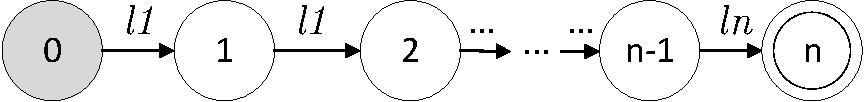
\includegraphics[scale=.6]{pictures/M0Automaton.pdf}
			\label{fig:am0a}
		}
		
		\subfloat[]{
			%\begin{tikzpicture}
			%\graph[nodes={circle, draw}, grow right=2.25cm, branch down=1.75cm]{
			%	0 -> ["$l_1, e$"] 1 -> ["$l_2, e$"] 2 -> ["$...$"] "n-1" -> ["$l_n, e$"] n};
			%\end{tikzpicture}
			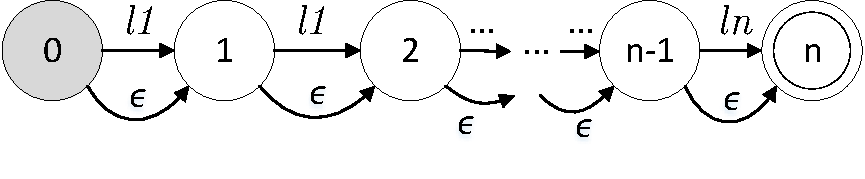
\includegraphics[scale=.6]{pictures/M0bAutomaton.pdf}
			\label{fig:am0b}
		}
		\caption{Автомат $M_0$ (a) и его замыкание (b).}
		\label{fig:am0}
	\end{figure}
	
	Полученный автомат порождает множество строк $L'$. Так, например, для строки $a12b$ искомое множество порождается автоматом $M_1$~(рис.~\ref{fig:M1}).
    \begin{figure}
    	\centering
    	%\begin{tikzpicture}
    	%\graph[nodes={circle, draw}, grow right=2.25cm, branch down=1.75cm]{
    	%	0 -> ["$a, e$"] 1 -> ["$1, e$"] 2 -> ["$2, e$"] "3" -> ["$b, e$"] 4};
    	%\end{tikzpicture}
    	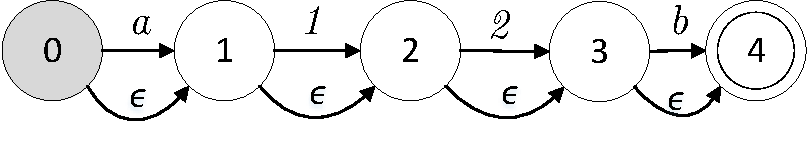
\includegraphics[scale=.6]{pictures/M1Automaton.pdf}
    	\caption{Автомат $M_1$ --- для строки $ a12b $.}
    	\label{fig:M1}
    \end{figure}
    
    Результатом работы алгоритма для каждой из грамматик со стартовым нетерминалом $A_i$ является лес разбора, описывающий
    искомое множество $T'_i$. Таким образом, после применения алгоритма, необходимо отыскать такие $T_1, T_2, ..., T_n$, что 
    будут выполнены следующие условия
    \begin{itemize}
    	\item $\forall T_i, i \in 1..n : T_i \in T'_i$;
    	\item объединение элементов крон $T_1, T_2, ..., T_n$ образует $L$;
    	\item порядок терминалов в кронах согласован с порядком в $L$;
    	\item пересечение элементов крон $T_1, T_2, ..., T_n$ --- $\epsilon$.
    \end{itemize}

	Представим эту задачу в форме задачи о выполнимости булевой формулы (SAT). 
	Для множества лесов разбора $T'_1, T'_2, ..., T'_n$ и входной строки $L$ формула состоит из двух
	частей связанных конъюнкцией($\&$). Первая часть состоит из конъюнкции формул описывающих
	каждый из лесов разбора $T'_i$, которая строится рекурсивно по структуре SPPF, псевдокод этой процедуры приведён в листинге~\ref{sppfToFormula}. 
	Имена переменных формируются из имён терминалов, их позиций во входной строке и номера текущего SPPF.
	Заметим, что для упакованного узла добавляются отрицания переменных, соответствующих терминалам которые не использованы в данном дереве.
	
	Вторая часть формулы описывает условие принадлежности каждого терминала ровно одному SPPF и имеет 
	следующий вид: $(t_1^j\ xor\ t_2^j\ xor\ ...\ xor\	 t_n^j)$, где $t_i^j$ --- терминал в позиции $i$ из SPPF $T'_j$.

	\begin{lstlisting}[caption={Функция SPPFtoFormula, преобразующая SPPF в булеву формулу},
	                   captionpos=b,
	                   label={sppfToFormula},
	                   language=Caml,
	                   basicstyle=\small]
 function nodeToFormula(node, SPPFn) =
   match node with
  | TerminalNode(terminal,(posL,posR)) ->
    Variable(SPPFn,terminal,posL))
  | NonterminalNode(children,_)
  | IntermediateNode(children,_) ->
    result = nodeToFormula(child[0])
    for child in children[1..length(children)] do
      result = AND(result, nodeToFormula(child))
    result
  | PackedNode(left,right,(posL,posR)) ->
    if (left != NULL)
    then
      result = AND(nodeToFormula(left), nodeToFormula(right))
      if (left.posR != right.posL)
      then
        for i in [left.posR..right.posL-1] do
          result = AND(result, NOT(Variable(SPPFn,input[i],i)))
      result
    else
      nodeToFormula(right)
 
function SPPFtoFormula(root : NonterminalNode, SPPFn) = 
  result = nodeToFormula(root, SPPFn)
  for i in [0 .. root.posL]@[root.posR .. input.Length] do
    result = AND(result, NOT(Variable(SPPFn,input[i],i)))
  result
   	\end{lstlisting}
	
	Описанная формула --- экземпляр задачи SAT. Решение полученной таким образом задачи SAT следует интерпретировать так.
	Если решение не может быть построено, то строка не принадлежит языку, который задан изначальной
	контекстно-свободной грамматикой с шаффлом. В случае существования множества решений $F$, 
	искомое множество деревьев разбора $R = \{T_1, T_2, ..., T_n\}$ может быть восстановлено. Для этого необходимо 
	извлечь из каждого SPPF $T'_j$ множество деревьев $T_j^f$, крона которых состоит из терминалов $t_i$ , таких, что 
	переменной $t_i^j $ в решении установлено значение истины. Этот процесс следует произвести для каждого из найденных решений.
	Тогда $R = \bigcup\limits_{f\in F} (T_1^f \bigtimes T_2^f \bigtimes ... \bigtimes T_n^f)$, где $F$ --- множество всех решений задачи SAT.
	Таким образом, получен алгоритм для решения задачи синтаксического анализа контекстно-свободных грамматик с шаффлом.
	
	\subsection{Применение анализа CFSG в распознавании планов}
	
	Предложенный алгоритм синтаксического анализа CFSG может использоваться в решении задачи распознавания планов.
	Для этого необходимо построить контекстно-свободную грамматику с шаффлом для библиотеки планов данной в задаче.
	Этот процесс осуществляется следующими шагами: 
	\begin{itemize}
		\item описанным ранее способом, построить для библиотеки планов множество контекстно-свободных грамматик со стартовыми нетерминалами $A_1...A_n$;
		\item создать продукцию вида $S \rightarrow A_1 \odot A_2 \odot ... \odot A_n$, где $S$ --- стартовый нетерминал CFSG, который не содержится в алфавите нетерминалов грамматик, построенных на предыдущем шаге.
	\end{itemize}

	После применения предложенного ранее алгоритма к этой грамматике и последовательности действий, будет получено множество решений ---
	наборов деревьев, которые описывают иерархию действий в соответствии с библиотекой планов.
	
	
	
	
	\section{Реализация алгоритма}
    
    Предложенный в данной работе алгоритм реализован на языке F\#, на базе проекта YaccConstructor. 
    Структура решения приведена в диаграмме изображённой на рис.~\ref{fig:diagram}.
    Выделенные модули были реализованы в рамках данной работы, алгоритм Generalised LL 
    был реализован в проекте и был переиспользован. Кроме того, для решения задачи SAT была использована библиотека
    ``Z3''~\cite{Z3} от Microsoft.
    \begin{figure}[H]
    	\centering
    	
    	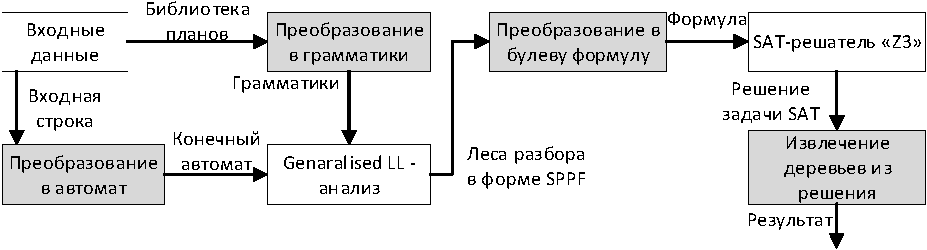
\includegraphics[scale=1.03]{pictures/diagram.pdf}
    	\caption{Структура реализации.}
    	\label{fig:diagram}
    \end{figure}

    \section{Эксперименты}
    На текущий момент наиболее производительным в решении задачи распознавания планов представляется алгоритм SLIM.
    В связи с этим было проведено сравнение времени работы описанного алгоритма со SLIM на одной библиотеке планов.
    Сравнение осуществлялось с результатами авторов предложенными в
    статье~\cite{mirsky2017slim}. Результаты представлены в таблице~\ref{expTable} (GLL + SAT --- результат данной работы) и показывают
    превосходство алгоритма предложенного в данной работе.
    
    \begin{table}[ht]   
    	\begin{center}
    		\begin{tabular}{ | c | c | c | c | c | c | c | c | c | c |  }
    			\hline
    			Кол-во действий & 1& 2& 3& 4& 5& 6& 7& 8& 9 \\
    			\hline
    			SLIM & 0.16 & 0.16 & 0.18 & 0.25 & 0.43 & 0.74 & 1.21 & 1.92 & 4.45 \\
   				GLL + SAT & 0.17 & 0.24 & 0.33& 0.38& 0.51& 0.62& 0.63& 1.19& 1.47\\
   				\hline
    		\end{tabular}
    	\end{center}
    	\caption{Время работы алгоритмов.}
    	\label{expTable}
    \end{table}
    
    \section{Результаты}
    В данной работе были получены следующие результаты.
    
    \begin{itemize}
    	\item Исследована возможность применения расширения алгоритма Generalised LL
    	      в задаче распознавания планов, путём комбинирования с SAT-решателем.
        \item Разработан алгоритм распознавания планов, на основе синтаксического анализа контекстно-свободных грамматик с шаффлом (CFSG).
              После предварительного сужения пространства поиска с помощью алгоритма Generalised LL, анализ производится SAT-решателем.
        \item Выполнена реализация предложенного подхода в рамках проекта YaccConstructor. Исходный код доступен
        в репозитории проекта: https://github.com/YaccConstructor/YaccConstructor
        \item Экспериментальное сравнение реализованного алгоритма с аналогом показало существенный прирост производительности. 
    \end{itemize}
    
   	\setmonofont[Mapping=tex-text]{CMU Typewriter Text}
    \bibliographystyle{ugost2008ls}
    \bibliography{diploma}
\end{document}
